\section{Data Free-ride Attack}
\label{sec:intro}
%new version, from Alfred
VoLTE transmits voice data through IP Multimedia Subsystem (IMS) in LTE network using a ``dedicated bearer'', which is a ``pipe line'' that transports data between the device and the gateways. Prior to VoLTE, all the application data is transmitted by a default bearer where QoS is not guaranteed.

\textbf{Attack Design. }Shown in Fig. 1, the two different bearers, a default one and a dedicated one, are implemented as two network interfaces on Android device, denoted as \texttt{IF0} and \texttt{IF1} respectively. The choice of interfaces to send a certain packet flow is controlled by the routing table on the device, where \texttt{IF0} is set to be used by default and \texttt{IF1} is used when the destination of the packets is the IMS nodes. We discovered that user with root privilege can send packets to arbitrary destinations using \texttt{IF1} by manipulating the routing table. These packets sent from \texttt{IF1} bypass the volume-based charge since they are carried by the voice channel, and also won't incur any time-based charge because no call session is initiated. We also unrevealed that downlink ICMP packets can be sent to \texttt{IF1} from third-party servers without getting blocked by the firewall or incurring any charge, which grants fraudulent user free uplink and downlink data access. Users can thus set up their own proxy to intercept device's HTTP request sent from \texttt{IF1}, fetch contents from the Internet and transmit data back to the \texttt{IF1} on the device using an ICMP tunnel, thus avoid charges.

\textbf{Validation.} We built a demo app to show the feasibility of downloading a 10 MB video within 2 seconds without data charge from the proxy server outside the cellular network and we measured that the downlink bandwidth of this free data channel can be up to 7 Mbps.

\begin{figure}[!t]
\hspace{-0.2in}
\centering
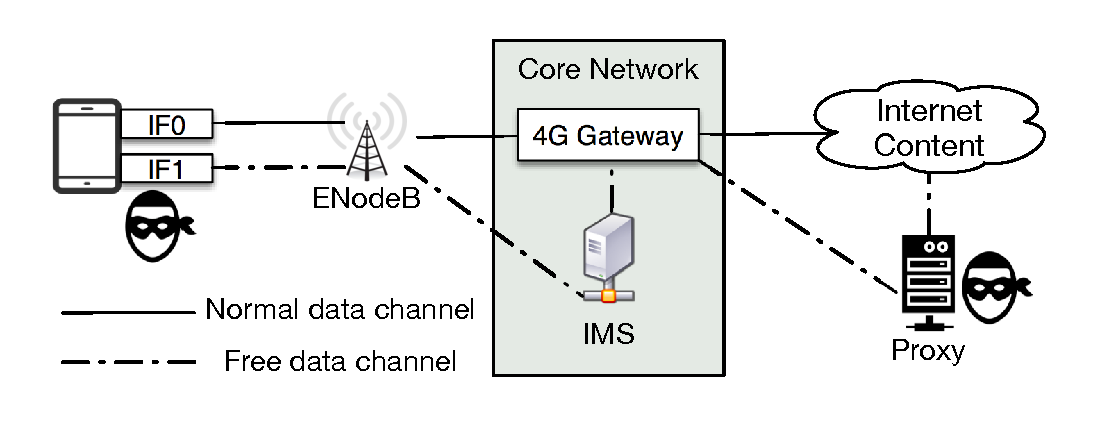
\includegraphics[width=3.3in]{figs/poster.eps}
\caption{VoLTE Data free-ride attack.}
\vspace{-0.1in}
\label{fig:attack}
\end{figure}
